%%%%%%%%%%%%%%%%%%%%%%%%%%%%%%%%%%%%%%%%%%%%%%%%%%%%%%%%%%%%%%%%%%%%%%%%%%%%%%%%%%%%%%%
%%%%%%%%%%%%%%%%%%%%%%%%%%%%%%%%%%%%%%%%%%%%%%%%%%%%%%%%%%%%%%%%%%%%%%%%%%%%%%%%%%%%%%%
% 
% This top part of the document is called the 'preamble'.  Modify it with caution!
%
% The real document starts below where it says 'The main document starts here'.

\documentclass[12pt]{article}

\usepackage{amssymb,amsmath,amsthm}
\usepackage[top=1in, bottom=1in, left=1.25in, right=1.25in]{geometry}
\usepackage{fancyhdr}
\usepackage{graphicx}
\usepackage{enumerate}
\usepackage{verbatim}
\usepackage{listings}
\usepackage{float}

% Comment the following line to use TeX's default font of Computer Modern.
\usepackage{times,txfonts}

\newtheoremstyle{homework}% name of the style to be used
  {18pt}% measure of space to leave above the theorem. E.g.: 3pt
  {12pt}% measure of space to leave below the theorem. E.g.: 3pt
  {}% name of font to use in the body of the theorem
  {}% measure of space to indent
  {\bfseries}% name of head font
  {:}% punctuation between head and body
  {2ex}% space after theorem head; " " = normal interword space
  {}% Manually specify head
\theoremstyle{homework} 

% Set up an Exercise environment and a Solution label.
\newtheorem*{exercisecore}{\@currentlabel}
\newenvironment{exercise}[1]
{\def\@currentlabel{#1}\exercisecore}
{\endexercisecore}

\newcommand{\localhead}[1]{\par\smallskip\noindent\textbf{#1}\nobreak\\}%
\newcommand\solution{\localhead{Solution:}}



% \newcommand{includematlab}[1]{\verbatiminput{#1}}

%%%%%%%%%%%%%%%%%%%%%%%%%%%%%%%%%%%%%%%%%%%%%%%%%%%%%%%%%%%%%%%%%%%%%%%%
%
% Stuff for getting the name/document date/title across the header
\makeatletter
\RequirePackage{fancyhdr}
\pagestyle{fancy}
\fancyfoot[C]{\ifnum \value{page} > 1\relax\thepage\fi}
\fancyhead[L]{\ifx\@doclabel\@empty\else\@doclabel\fi}
\fancyhead[C]{\ifx\@docdate\@empty\else\@docdate\fi}
\fancyhead[R]{\ifx\@docauthor\@empty\else\@docauthor\fi}
\headheight 15pt

\def\doclabel#1{\gdef\@doclabel{#1}}
\doclabel{Use {\tt\textbackslash doclabel\{MY LABEL\}}.}
\def\docdate#1{\gdef\@docdate{#1}}
\docdate{Use {\tt\textbackslash docdate\{MY DATE\}}.}
\def\docauthor#1{\gdef\@docauthor{#1}}
\docauthor{Use {\tt\textbackslash docauthor\{MY NAME\}}.}
\makeatother

%% General formatting parameters
\parindent 0pt
\parskip 12pt plus 1pt

\def\vx{\mathbf x}
\def\vb{\mathbf b}

% Shortcuts for blackboard bold number sets (reals, integers, etc.)
\newcommand{\Reals}{\ensuremath{\mathbb R}}
\newcommand{\Nats}{\ensuremath{\mathbb N}}
\newcommand{\Ints}{\ensuremath{\mathbb Z}}
\newcommand{\Rats}{\ensuremath{\mathbb Q}}
\newcommand{\Cplx}{\ensuremath{\mathbb C}}
%% Some equivalents that some people may prefer.
\let\RR\Reals
\let\NN\Nats
\let\II\Ints
\let\CC\Cplx

%%%%%%%%%%%%%%%%%%%%%%%%%%%%%%%%%%%%%%%%%%%%%%%%%%%%%%%%%%%%%%%%%%%%%%%%%%%%%%%%%%%%%%%
%%%%%%%%%%%%%%%%%%%%%%%%%%%%%%%%%%%%%%%%%%%%%%%%%%%%%%%%%%%%%%%%%%%%%%%%%%%%%%%%%%%%%%%
% 
% The main document start here.

% The following commands set up the material that appears in the header.

%%%%%%%%%%%%%%%%%%%%%%%%%%%%%%%%%%%%%%%%%%%%%%%%%%%%%%%%%%%%%%%%%%%%%%%%%%
\doclabel{Math 426: Homework 10}
\docauthor{Stefano Fochesatto}
\docdate{November 4, 2020}

\begin{document}

\begin{exercise}{Supplemental 1}
Consider these three points: $\{(1, 1), (2.5, 8), (4, 5)\}$.
Find the polynomial $P(x)$ of degree 2 which passes through these points. Do this three different ways, by using
\begin{enumerate}
\item[(a)] the Vandermonde matrix method,
\solution By the Vandermonde matrix method we can solve for the coefficients of $P(x)$ by solving the following system,
\begin{equation*}
  \begin{pmatrix}
    1&& 1 && 1 \\
    1 && 2.5 && 2.5^2 \\
    1&& 4 && 4^2 
  \end{pmatrix}
  \begin{pmatrix}
    c_0 \\
    c_1 \\
    c_2 
  \end{pmatrix}
   = 
   \begin{pmatrix}
    1 \\
    8 \\
    5 
  \end{pmatrix}
\end{equation*}
Solving with MATLAB we get,\\
\textbf{Console:}
\begin{center}
\lstinputlisting{vandermonde.txt}
\end{center}
This gives us that our polynomial is,
\begin{equation*}
  P(x) = -2.22x^2 + 12.44x - 9.22
\end{equation*}
\vspace{.25in}


\item[(b)] The Newton form and its triangular matrix method\\
\solution The Newton Form of the interpolation polynomial is,
\begin{equation*}
  P(x) = c_0 + c_1(x - x_0) + c_2(x - x_0)(x - x_1)
\end{equation*}
Applying $P(x_i) = y_i$ and solving for $c_i$ is the same as solving the lower triangular system 
\begin{equation*}
  \begin{pmatrix}
    1&& 0 && 0 \\
    1 && 2.5 - 1 && 0 \\
    1&& 4 - 1 && (4 - 1)(4 - 2.5) 
  \end{pmatrix}
  \begin{pmatrix}
    c_0 \\
    c_1 \\
    c_2 
  \end{pmatrix}
   = 
   \begin{pmatrix}
    1 \\
    8 \\
    5 
  \end{pmatrix}
\end{equation*}
Solving with MATLAB we get,\\
\textbf{Console:}
\begin{center}
\lstinputlisting{newton.txt}
\end{center}
Substituting our coefficients in the Newton Form,
\begin{equation*}
  P(x) = 1.0  + 4.66 (x - 1) - 2.222(x - 1)(x - 2.5).
\end{equation*}
\vspace{.25in}




\item[(c)] the Lagrange form.\\
\solution We can easily write the basis functions $\phi(x)$ for the lagrange form polynomial $P(x)$,
\begin{equation*}
  \phi_0(x) = \dfrac{(x - 2.5)(x - 4)}{(1 - 2.5)(1 - 4)}
\end{equation*}
\begin{equation*}
  \phi_1(x) = \dfrac{(x - 1)(x - 4)}{(2.5 - 1)(2.5 - 4)}
\end{equation*}
\begin{equation*}
  \phi_2(x) = \dfrac{(x - 1)(x - 2.5)}{4 - 1)(4 - 2.5)}
\end{equation*}
Following the Lagrange Form for the interpolation polynomial,
\begin{align*}
  P(x) &= \sum_{k = 0}^n y_k \phi_k(x),\\
  P(x) &= \dfrac{(x - 2.5)(x - 4)}{(1 - 2.5)(1 - 4)} + 8\dfrac{(x - 1)(x - 4)}{(2.5 - 1)(2.5 - 4)} + 5\dfrac{(x - 1)(x - 2.5)}{4 - 1)(4 - 2.5)},
\end{align*}
\end{enumerate}
\end{exercise}
\vspace{.5in}






\begin{exercise}{Supplemental 2}
Consider the $x$ coordinates $x_0=0$, $x_1=\pi/3$, $x_2=2\pi/3$ and $x_3=\pi$.
\begin{enumerate}
	\item[a)] Plot the four Lagrange basis functions $\phi_k$ $k=0,\ldots,4$ on a single graph with domain $[0,\pi]$.\\
  \solution
  \textbf{Console:}
  \begin{center}
  \lstinputlisting{LagrangeBasis.txt}
  \end{center}
  
  \begin{figure}[H]
   \caption{Plot of the Lagrange Basis Functions}
   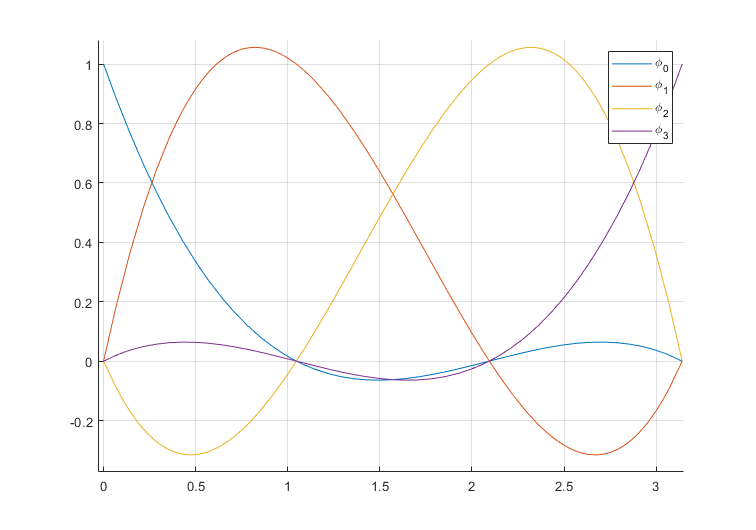
\includegraphics[width = \textwidth]{Basisplot.png}  
   \centering
\end{figure}

  
  



	\item[b)] Plot the four Newton interpolation basis functions
  $\psi_k$, each on its own individual graph.\\

  \solution 
  \textbf{Console:}
  \begin{center}
  \lstinputlisting{Newtonbasis.txt}
  \end{center}

  \begin{figure}[H]
    \caption{Plot of $\psi_0$}
    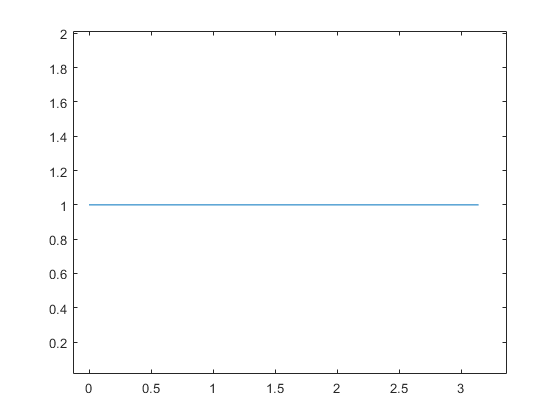
\includegraphics[width = .60\textwidth]{newtonbasis1.png}  
    \centering
 \end{figure}

 \begin{figure}[H]
  \caption{Plot of $\psi_1$}
  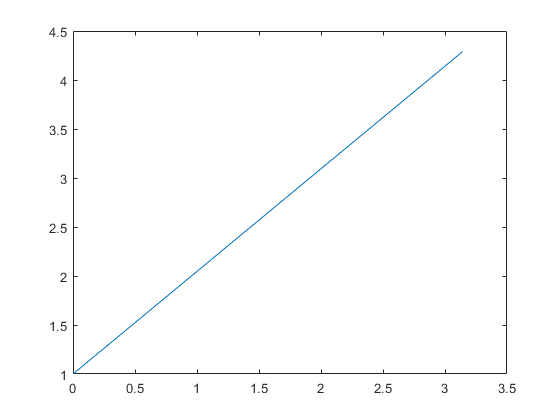
\includegraphics[width = .60\textwidth]{newtonbasis2.png}  
  \centering
\end{figure}


\begin{figure}[H]
  \caption{Plot of $\psi_2$}
  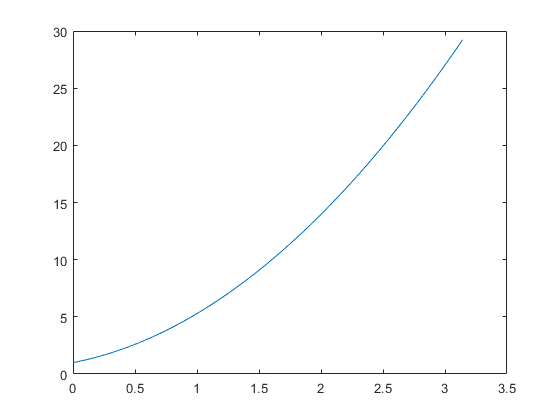
\includegraphics[width = .60\textwidth]{newtonbasis3.png}  
  \centering
\end{figure}


\begin{figure}[H]
  \caption{Plot of $\psi_3$}
  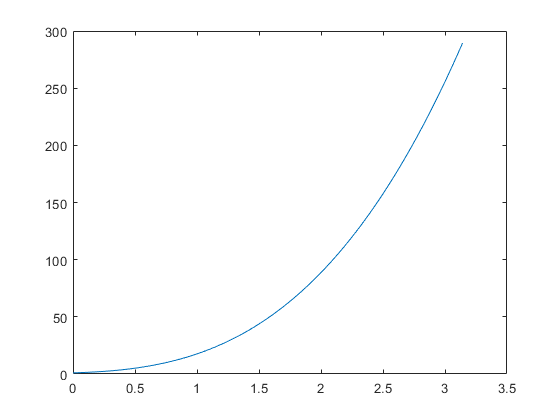
\includegraphics[width = .60\textwidth]{newtonbasis4.png}  
  \centering
\end{figure}







	\item[c)] Plot the graph of $\sin(x)$ along with its Lagrange interpolant $p_{\mathrm{Lag}}$.\\ 
  \solution
  \textbf{Console:}
  \begin{center}
  \lstinputlisting{Lagrangeinter.txt}
  \end{center}
  \begin{figure}[H]
    \caption{Plot of $p_{\mathrm{Lag}}$ and $sin(x)$}
    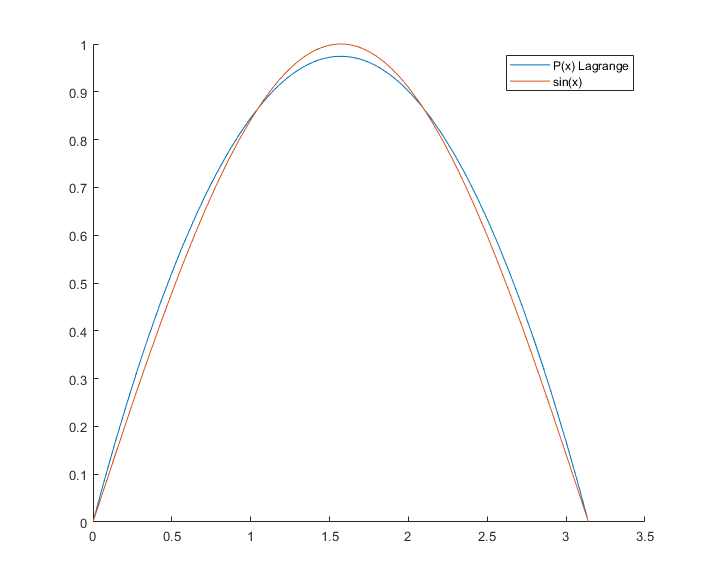
\includegraphics[width = .75\textwidth]{LagrangeInter.png}  
    \centering
  \end{figure}
  
  
  


	\item[d)] Plot the graph of $\sin(x)$ along with its Newton interpolant $p_{\mathrm{Newt}}$.\\
  \solution 
  \textbf{Console:}
  \begin{center}
  \lstinputlisting{NewtonInter.txt}
  \end{center}
  \begin{figure}[H]
    \caption{Plot of $p_{\mathrm{Newt}}$ and $sin(x)$}
    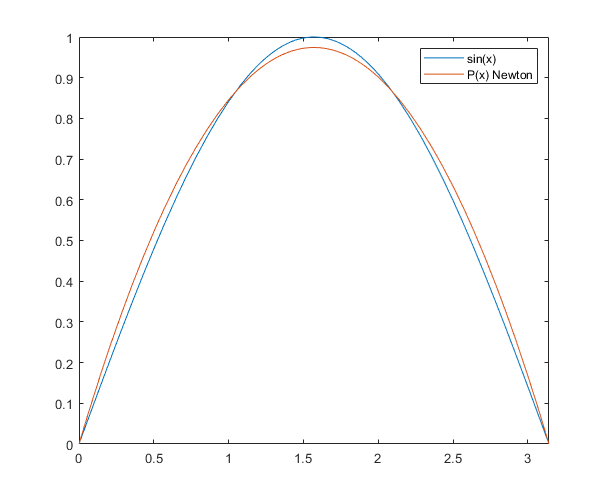
\includegraphics[width = .75\textwidth]{NewtonInter.png}  
    \centering
  \end{figure}
  
  




	\item[e)] What is the relative error of $p_{\mathrm{Lag}}(\pi/4)$?\\
  \solution The relative error of our lagrange interpolant at a given point $x$ is calculated by,
  \begin{equation*}
    e_{relative} = |\dfrac{sin(x) - p_{\mathrm{Lag}}(x)}{sin(x)}|,
  \end{equation*}
  \textbf{Console:}
  \begin{center}
  \lstinputlisting{error.txt}
  \end{center}
\end{enumerate}
\end{exercise}
\vspace{.5in}






\begin{exercise}{Exercise 8.1}
  \begin{enumerate}
    \item Plot population versus years  after 1900 using MATLAB by entering the years after 1900 into a vector \dots 
    \solution 
    \textbf{Console:}
  \begin{center}
  \lstinputlisting{Census.txt}
  \end{center}
  
  \begin{figure}[H]
    \caption{Census Extrapolation with Vandermonde Interpolation (red)}
    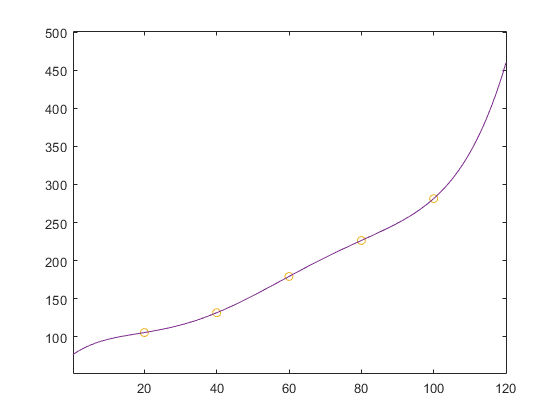
\includegraphics[width = .80\textwidth]{Census.png}  
    \centering
  \end{figure}
  \vspace{.25in}


  \item  Write down the Lagrange form of the second­
  degree polynomial that interpolates the population in the years 1900, 1920, and 1940.\\

  \solution From the definition we know that the Lagrange form of the second­ degree polynomial is,
  \begin{equation*}
    p_{\mathrm{Lag}} =  76 \dfrac{(x - 20)(x - 40)}{(0 - 20)(0 - 40)} + 105.7 \dfrac{(x - 0)(x - 40)}{(20 - 0)(20 - 40)} + 131.7\dfrac{(x - 0)(x - 20)}{(40 - 0)(40 - 20)},
  \end{equation*} 
  \vspace{.25in}
  



\item Determine the coefficients of the Newton form of the interpolants of degrees 0, 1, and 2, that
 interpolate the first one, two, and three data points, respectively. 
Verify that the second­ degree polynomial that you construct here is identical to part 2\\
\solution Using MATLAB to find the coefficients for the newton interpolants of degree 0,1,2 for the first three data points of the census.\\ 
\textbf{Console:}
\begin{center}
\lstinputlisting{Quicknewtons.txt}
\end{center}
\end{enumerate}
\end{exercise}





\begin{exercise}{Exercise 8.2} Called Muller’s method, fits a quadratic through the three points, $(x_{k−2}, (x_{k−2}))$, $(x_{k−1}, (x_{k−1}))$, and  $(x_k, f(x_k))$,  and  takes the  root  of  this  quadratic that  is closest to $x_k$ as the next approximation $x_{k+1}$. Write down a formula for this quadratic. Suppose $f(x) = x^3 - 2$, $x_0 = 0$, $x_1 = 1$, and $x_2 = 2$. Find $x_3$
  \solution Using a Vandermonde interpolation we can find the formula for the Muller quadratic,\\
  \textbf{Console:}
\begin{center}
\lstinputlisting{vanderquick.txt}
\end{center}
We get a polynomial, 
\begin{equation*}
  P(x) = 2x^2 - 2x - 2.
\end{equation*}
Using the secant method we can rootfind, and we get that the next value is $x_3 = 1.61802$,\\
\textbf{Console:}
\begin{center}
\lstinputlisting{root.txt}
\end{center}


  




\end{exercise}

\end{document}